% Solving Reflected Diffusion Models: A Physics-Informed Approach
% A diffusion path reflects off the domain boundary; a physics-informed network fits the density over collocation points.
% Below the drawing: the reflected SDE, the Fokker-Planck equation with its zero-flux (Neumann) boundary
% condition, and the PINN training loss, as stated in the paper (Sections 2-3).
\documentclass[border=0pt]{standalone}
\usepackage{tikz}
% Shared look for the TikZ publication thumbnails.
% Canvas: 16cm x 10cm (16:10, matching the 640x400 WebP output), white, site palette.
% Labels are large (\lbl) because thumbnails are shown about 200px wide.
\usepackage[T1]{fontenc}
\usepackage{helvet}
\renewcommand{\familydefault}{\sfdefault}
\usepackage{amsmath,amssymb}
\usepackage{fontawesome5}
\usetikzlibrary{arrows.meta,calc,positioning,shapes.geometric,shapes.callouts,decorations.pathmorphing,shadows}

\definecolor{ink}{HTML}{2B2D42}
\definecolor{accent}{HTML}{B509AC}
\definecolor{teal}{HTML}{1E9BC0}
\definecolor{violet}{HTML}{6C5CE7}
\definecolor{orange}{HTML}{F28C28}
\definecolor{sun}{HTML}{F2C14E}
\definecolor{leaf}{HTML}{2CA58D}
\definecolor{alert}{HTML}{E5484D}
\definecolor{mist}{HTML}{EEF0F5}

\tikzset{
  every picture/.append style={line cap=round, line join=round},
  card/.style={rounded corners=10pt, draw=#1!75!black, line width=1.4pt, fill=#1!12},
  arrow/.style={-{Stealth[length=10pt,width=9pt]}, line width=2.2pt, draw=#1},
  soft shadow/.style={drop shadow={shadow xshift=0pt, shadow yshift=-3pt, opacity=0.18, fill=ink}},
  badge/.style={circle, fill=#1!14, draw=#1, line width=2pt, minimum size=2.3cm, text=#1},
}
\newcommand{\thumbcanvas}{\useasboundingbox[fill=white] (0,0) rectangle (16,10);}
\newcommand{\lbl}[1]{{\fontsize{20}{22}\selectfont\bfseries #1}}
\newcommand{\icon}[2][34]{{\fontsize{#1}{#1}\selectfont\faIcon{#2}}}
% Window chrome: dark editor panel with traffic-light dots. Args: x0, y0, x1, y1.
\newcommand{\editor}[4]{%
  \fill[ink, rounded corners=12pt, soft shadow] (#1,#2) rectangle (#3,#4);
  \foreach \c [count=\k] in {alert,sun,leaf} \fill[\c] ({#1+0.15+0.42*\k},{#4-0.42}) circle (0.13);
}

\newsavebox{\drawing}
\begin{document}
\sbox{\drawing}{%
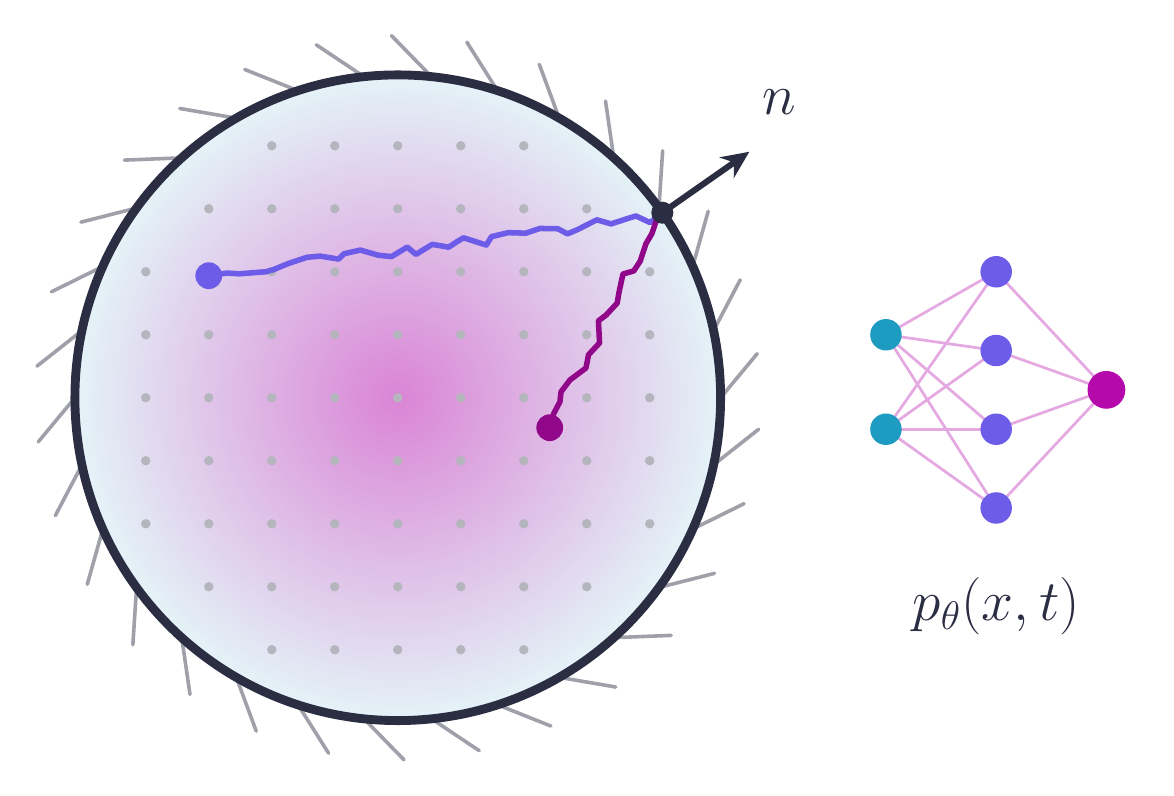
\begin{tikzpicture}
\useasboundingbox (0.7,0.3) rectangle (14.9,9.7);
% Domain with a density inside.
\shade[inner color=accent!50, outer color=teal!12] (5.4,5.0) circle (4.1);
\foreach \x in {2.2,3.0,...,8.7} \foreach \y in {1.8,2.6,...,8.3} {
  \pgfmathtruncatemacro{\inside}{((\x-5.4)^2+(\y-5.0)^2 < 13.5) ? 1 : 0}
  \ifnum\inside=1 \fill[ink!35] (\x,\y) circle (0.06); \fi
}
% Reflecting boundary.
\foreach \a in {0,12,...,348} \draw[ink!45, line width=1.3pt] ($(5.4,5.0)+(\a:4.1)$) -- ($(5.4,5.0)+(\a+7:4.6)$);
\draw[ink, line width=3.2pt] (5.4,5.0) circle (4.1);
% A sample path hits the boundary and reflects.
\pgfmathsetseed{11}
\draw[violet, line width=2pt, decorate, decoration={random steps, segment length=5pt, amplitude=2.5pt}] (3.0,6.55) -- (8.70,7.30);
\draw[accent!80!black, line width=2pt, decorate, decoration={random steps, segment length=5pt, amplitude=2.5pt}] (8.70,7.30) -- (7.33,4.62);
\fill[violet] (3.0,6.55) circle (0.17);
\fill[accent!80!black] (7.33,4.62) circle (0.17);
\fill[ink] (8.76,7.35) circle (0.14);
\draw[arrow=ink] (8.76,7.35) -- ++(35:1.35);
\node[text=ink] at (10.25,8.75) {\lbl{$n$}};
% Physics-informed network for the density.
\foreach \ya in {4.6,5.8} \foreach \yb in {3.6,4.6,5.6,6.6} \draw[accent!35, line width=1pt] (11.6,\ya) -- (13.0,\yb);
\foreach \yb in {3.6,4.6,5.6,6.6} \draw[accent!35, line width=1pt] (13.0,\yb) -- (14.4,5.1);
\foreach \ya in {4.6,5.8} \fill[teal] (11.6,\ya) circle (0.2);
\foreach \yb in {3.6,4.6,5.6,6.6} \fill[violet] (13.0,\yb) circle (0.2);
\fill[accent] (14.4,5.1) circle (0.24);
\node[text=ink] at (13.0,2.35) {\lbl{$p_\theta(x,t)$}};
\end{tikzpicture}}%
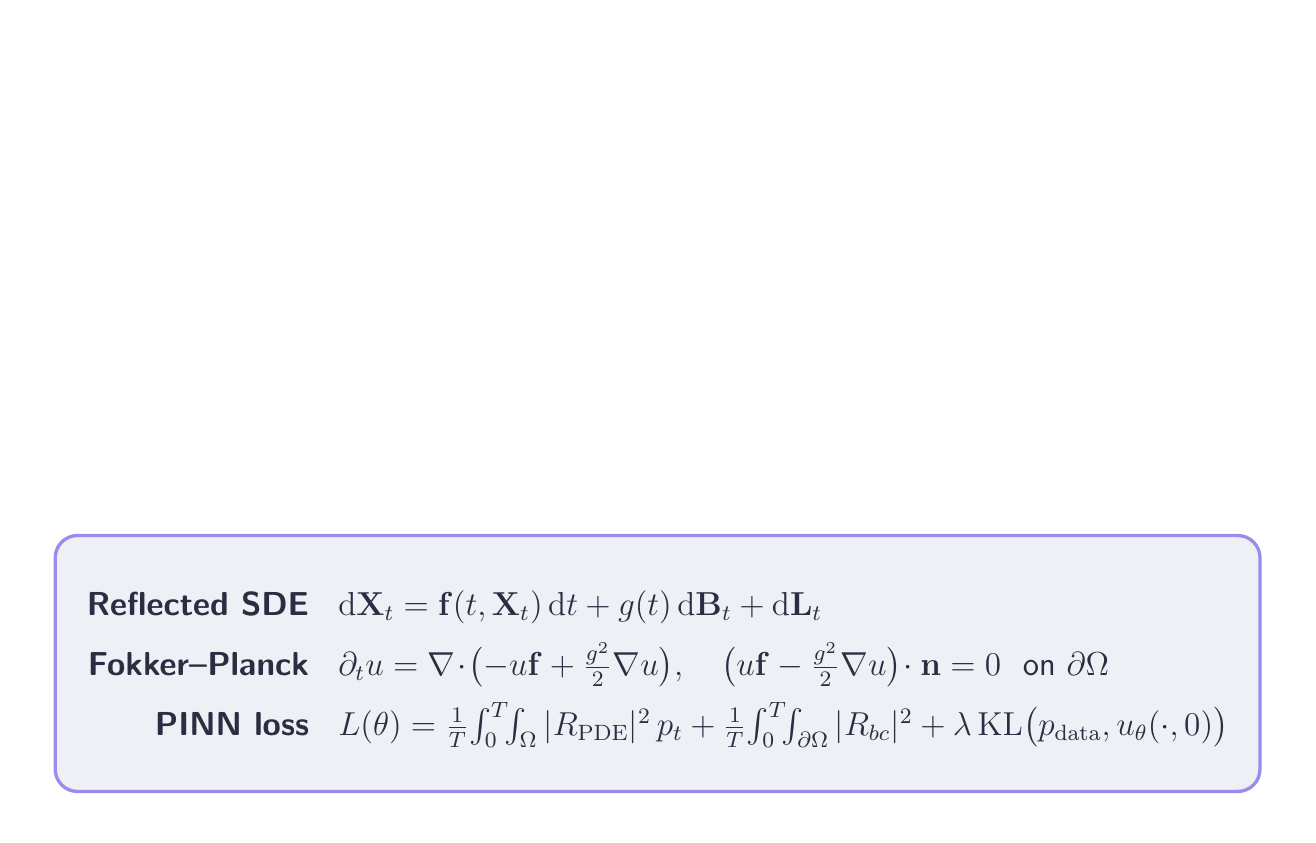
\begin{tikzpicture}
\thumbcanvas
% The drawing, scaled uniformly (line widths included) into the top of the canvas.
\node[inner sep=0pt] at (8,6.85) {\scalebox{0.64}{\usebox{\drawing}}};
% Key equations.
\fill[mist, rounded corners=8pt] (0.35,0.3) rectangle (15.65,3.55);
\draw[violet!70, line width=1.2pt, rounded corners=8pt] (0.35,0.3) rectangle (15.65,3.55);
\node[text=ink, font=\fontsize{12}{14}\selectfont] at (8,1.925) {%
  \renewcommand{\arraystretch}{1.55}%
  \begin{tabular}{@{}r@{\hspace{0.9em}}l@{}}
  \textbf{Reflected SDE} &
  $\mathrm{d}\mathbf{X}_t=\mathbf{f}(t,\mathbf{X}_t)\,\mathrm{d}t+g(t)\,\mathrm{d}\mathbf{B}_t+\mathrm{d}\mathbf{L}_t$\\
  \textbf{Fokker--Planck} &
  $\partial_t u=\nabla\!\cdot\!\big({-u\mathbf{f}}+\tfrac{g^2}{2}\nabla u\big),\quad
   \big(u\mathbf{f}-\tfrac{g^2}{2}\nabla u\big)\!\cdot\mathbf{n}=0\ \ \text{on }\partial\Omega$\\
  \textbf{PINN loss} &
  $L(\theta)=\frac{1}{T}\!\int_0^T\!\!\int_\Omega |R_{\mathrm{PDE}}|^2\,p_t
   +\frac{1}{T}\!\int_0^T\!\!\int_{\partial\Omega} |R_{bc}|^2
   +\lambda\,\mathrm{KL}\big(p_{\mathrm{data}},u_\theta(\cdot,0)\big)$
  \end{tabular}};
\end{tikzpicture}
\end{document}
